\documentclass[aspectratio=169,11pt]{beamer}
\usepackage[utf8]{inputenc}
\usepackage[T1]{fontenc}
\usepackage[spanish]{babel}
\usepackage{amsmath,amssymb}
\usepackage{tikz}
\usetikzlibrary{arrows.meta,angles,calc,positioning}
\usetheme{Madrid}
\usecolortheme{default}
\setbeamertemplate{navigation symbols}{}
\setbeamertemplate{blocks}[rounded][shadow=false]
\newcommand{\ang}[1]{\angle #1^\circ}

\title[Dos caminos digitales]{Paso 11: Dos caminos para el QFT digital}
\subtitle{Diseñar en $z$ (Nichols directo) o en $w$ (Bode otra vez)}
\author{Curso de control robusto (QFT)}
\date{}
\begin{document}
\begin{frame}\titlepage\end{frame}

\begin{frame}{Dónde encaja este paso}
  \tiny
  \begin{enumerate}\setlength{\itemsep}{-2pt}
    \item[1.] Números complejos \hfill \textcolor{gray}{(hecho)}
    \item[2.] Funciones de transferencia: $s$, polos y ceros \hfill \textcolor{gray}{(hecho)}
    \item[3.] Respuesta en frecuencia: $s=j\omega$, magnitud y fase \hfill \textcolor{gray}{(hecho)}
    \item[4.] Decibelios y escala logarítmica (Bode) \hfill \textcolor{gray}{(hecho)}
    \item[5.] Realimentación: $L$, $T=\frac{L}{1+L}$, $S=\frac{1}{1+L}$ \hfill \textcolor{gray}{(hecho)}
    \item[6.] Nichols chart \hfill \textcolor{gray}{(hecho)}
    \item[7.] Incertidumbre y templates \hfill \textcolor{gray}{(hecho)}
    \item[8.] Especificaciones $\rightarrow$ bounds \hfill \textcolor{gray}{(hecho)}
    \item[9.] Loop shaping, prefiltro y verificación \hfill \textcolor{gray}{(hecho)}
    \item[10.] QFT en control digital \hfill \textcolor{gray}{(hecho)}
    \item[\textbf{11.}] \textbf{Dos caminos digitales: $z$ y $w$} \hfill $\leftarrow$ estamos aquí
    \item[12.] Estabilidad, límites, más especificaciones y caso real
    \item[13.] Muestreo por eventos con periodo base $T$
    \item[14.] Sistemas de dos estados: lazo interno y externo
    \item[15.] QFT y sistemas no lineales
    \item[16.] Algoritmos de QFT: cómo funcionan por dentro
    \item[17.] QFT en Python: una biblioteca paso a paso
    \item[18.] QFT en MATLAB: el mismo código, otra sintaxis
    \item[19.] Historia, panorama y bibliografía
  \end{enumerate}
  \vspace{2pt}
  \begin{block}{Objetivo de hoy}
    Hacer el \textbf{mismo diseño digital} ($T_s=0.05$ s, mismas especificaciones del paso 8) por dos caminos, y ver qué ve el diseñador en cada uno. Ambos son ``diseño directo en discreto'' del paso 10; la emulación queda aparte.
  \end{block}
\end{frame}

\begin{frame}{La pregunta: ¿hay un Bode y un Nichols digitales?}
  \small
  \begin{block}{Camino $z$: Nichols directo}
    Se evalúa $L(e^{j\omega T_s})$ para $0<\omega\le\omega_N=\pi/T_s$ y se dibuja en la carta de Nichols. Los templates, bounds y la verificación son los de los pasos 7--9, con $P_i(z)$ en vez de $P_i(s)$.
  \end{block}
  \begin{block}{Camino $w$: plano $w$ (Bode otra vez)}
    Con $w=\frac{2}{T_s}\frac{z-1}{z+1}$ todo vuelve a ser racional en una variable continua $w=j\nu$. Se pueden aplicar las reglas de Bode (ganancia, polos, ceros) y luego volver a $z$.
  \end{block}
  \begin{alertblock}{Lo importante}
    Los dos caminos trabajan con \textbf{los mismos números complejos}: solo cambia la etiqueta de frecuencia ($\omega$ o $\nu$) y las herramientas con las que se mueve la curva.
  \end{alertblock}
\end{frame}

\begin{frame}{Un número complejo, dos nombres: $\omega$ y $\nu$}
  \footnotesize
  \begin{columns}[T]
  \begin{column}{0.5\textwidth}
    Con $z=e^{j\omega T_s}$ y $w=\frac{2}{T_s}\frac{z-1}{z+1}$:
    \[ w=j\nu,\qquad \nu=\frac{2}{T_s}\tan\frac{\omega T_s}{2} \]
    Por tanto $L_z(e^{j\omega T_s})=L_w(j\nu)$: es \textbf{el mismo punto} del Nichols.
    \begin{itemize}
      \item $\omega$ llega solo hasta $\omega_N=\pi/T_s=62.8$ rad/s.
      \item $\nu$ llega hasta $\infty$ (Nyquist $\leftrightarrow\nu\to\infty$).
      \item Para $\omega T_s$ pequeño, $\nu\approx\omega$.
    \end{itemize}
  \end{column}
  \begin{column}{0.46\textwidth}
    $T_s=0.05$ s:
    \begin{center}
    \begin{tabular}{r|r|r}
      $\omega$ & $\nu$ & $\nu/\omega-1$\\\hline
      $1$ & $1.00$ & $0\%$\\
      $5$ & $5.03$ & $0.5\%$\\
      $10$ & $10.2$ & $2\%$\\
      $20$ & $21.9$ & $9\%$\\
      $30$ & $37.3$ & $24\%$\\
      $40$ & $62.3$ & $56\%$\\
      $50$ & $120$ & $141\%$\\
      $60$ & $564$ & $840\%$
    \end{tabular}
    \end{center}
  \end{column}
  \end{columns}
\end{frame}

\begin{frame}{El ejemplo que no cambia}
  \small
  \begin{itemize}
    \item Planta: $P(s)=\dfrac{K}{s(s+a)}$ con $K\in[1,5]$, $a\in[1,3]$; nominal $K=1$, $a=1$.
    \item Especificaciones del paso 8: estabilidad $|T|\le1.2$, seguimiento entre $T_L$ y $T_U$, rechazo $|S|\le W_d$.
    \item Se implementa con ZOH y $T_s=0.05$ s ($\omega_N=62.8$ rad/s). Las especificaciones se piden hasta $\omega=40$ rad/s.
    \item \textbf{Por qué este $T_s$}: es el caso del paso 10 donde el $G$ emulado \textbf{no} cumple ($\max|T|=3.51$ dB $>1.58$ dB) y hay que rediseñar.
  \end{itemize}
  \begin{block}{Qué se va a obtener}
    Un $G$ de adelanto $G=k\,\dfrac{1+s/z_0}{1+s/p_0}$, con $k$, $z_0$, $p_0$ por determinar, y un prefiltro $F$, comprobados en frecuencia y en el tiempo.
  \end{block}
\end{frame}

\section{Camino z}
\begin{frame}{Camino $z$: la receta}
  \small
  \begin{enumerate}
    \item Para cada $P_i$ de la familia: $P_i(z)=\mathcal{Z}\{\mathrm{ZOH}\cdot P_i(s)\}$ y se evalúa en $z=e^{j\omega_kT_s}$.
    \item Templates y bounds con la regla de siempre (pasos 7 y 8), a las frecuencias $\omega_k\le40$.
    \item Loop shaping: se elige $G(z)$ (polos y ceros en el plano $z$) y se mira dónde cae $L_0(e^{j\omega_kT_s})$ en el Nichols.
    \item Verificación hasta Nyquist, en frecuencia y en el tiempo.
  \end{enumerate}
  \begin{block}{Ventajas}
    El ZOH y el $T_s$ ya están dentro de $P_i(z)$. Las especificaciones se evalúan en las $\omega$ de verdad. No hay conversión de frecuencias.
  \end{block}
  \begin{alertblock}{Inconveniente}
    Las reglas de Bode asintótico (``un cero sube $+20$ dB/dec'') \textbf{no} valen en $z$. Hay que apoyarse en el Nichols o en una optimización.
  \end{alertblock}
\end{frame}

\begin{frame}{Camino $z$: el ``Bode'' digital existe, pero se curva}
  \footnotesize
  \begin{columns}[T]
  \begin{column}{0.58\textwidth}
    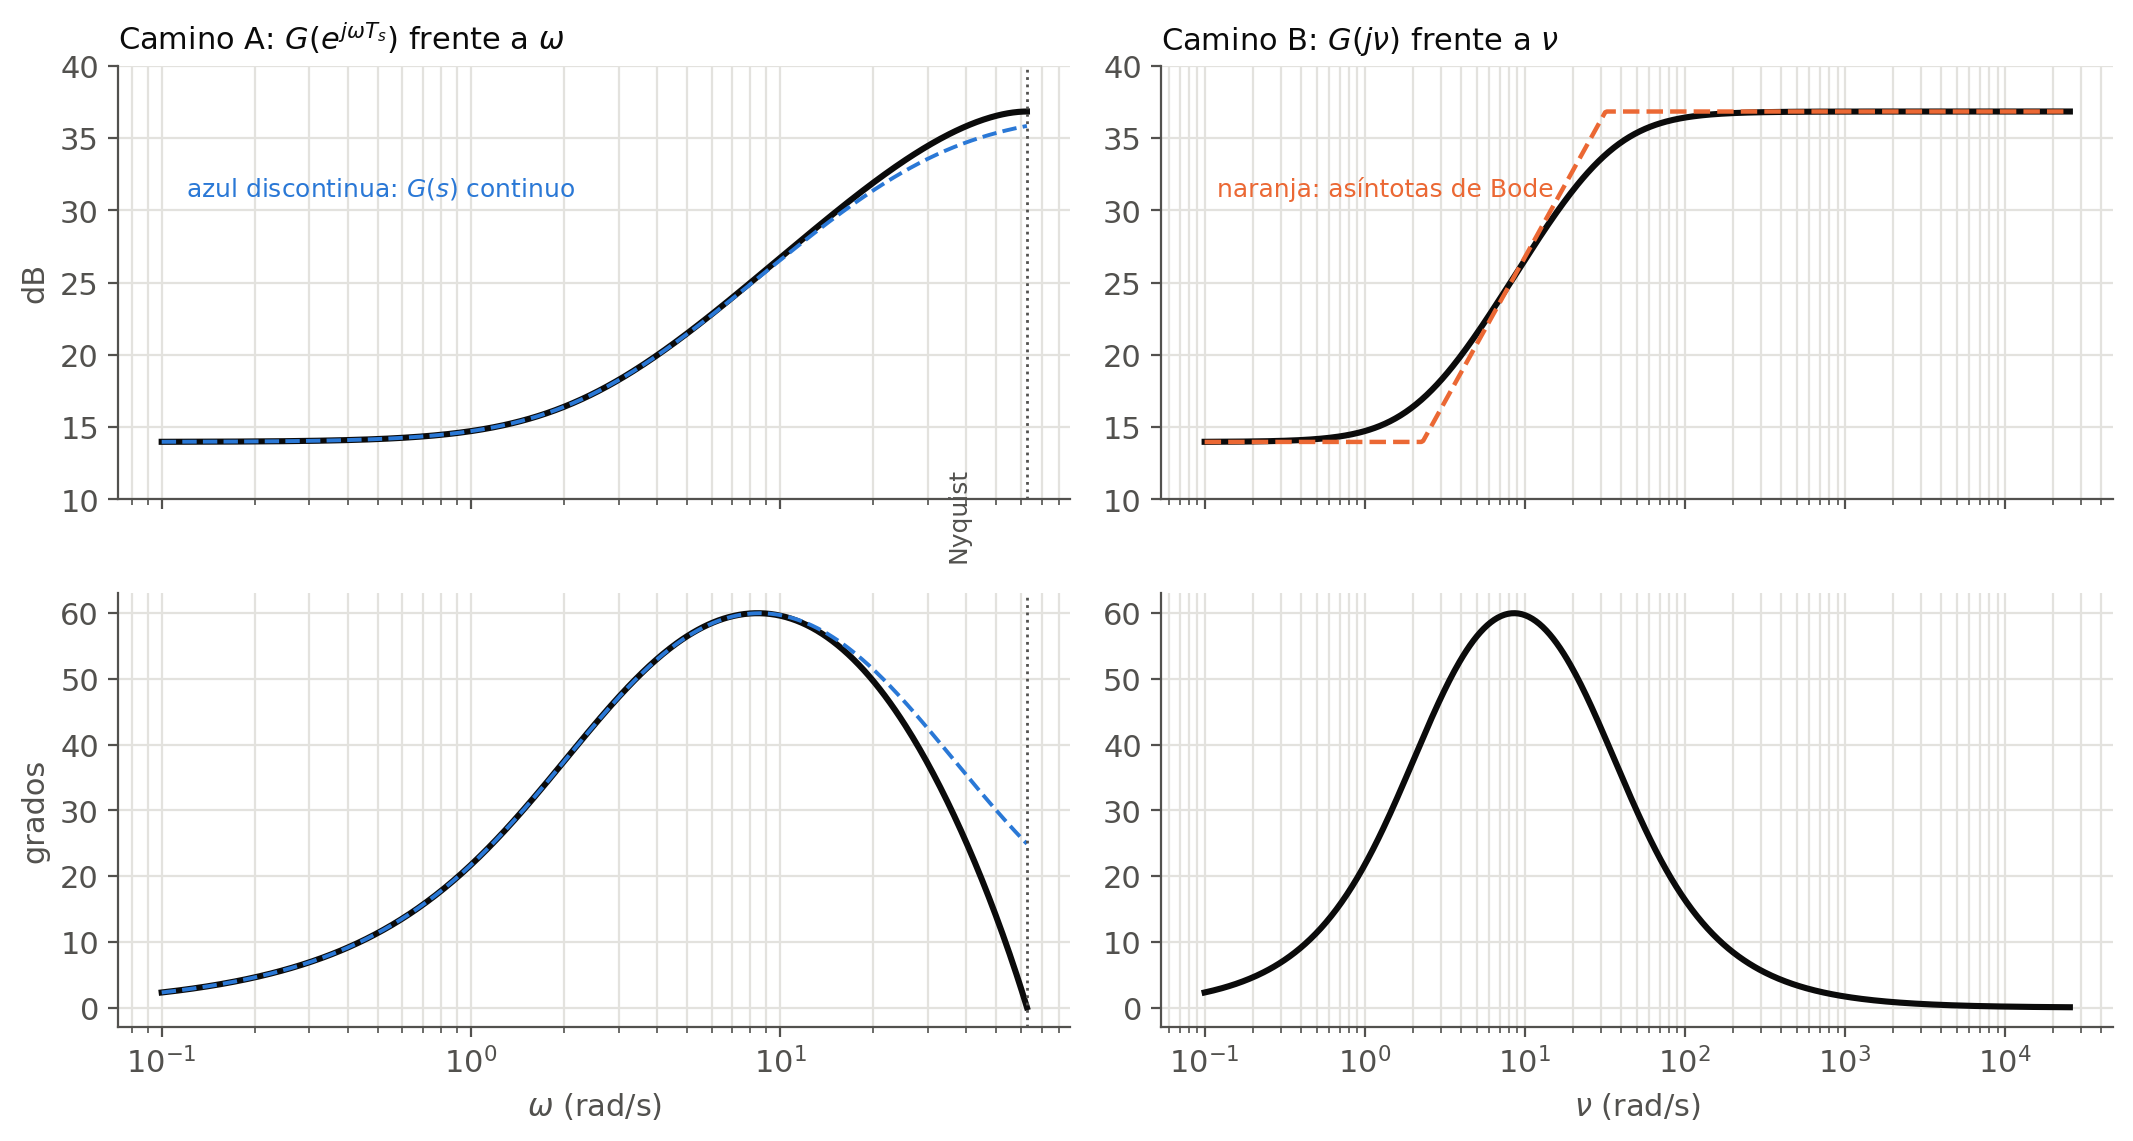
\includegraphics[width=\textwidth]{fig/bode_zw.png}
  \end{column}
  \begin{column}{0.4\textwidth}
    Izquierda: $|G(e^{j\omega T_s})|$ y fase frente a $\omega$, con el eje logarítmico acabado en Nyquist.
    \begin{itemize}
      \item Casi igual al $G(s)$ continuo (discontinuo) a baja frecuencia.
      \item Cerca de Nyquist, la fase \textbf{cae a $0^\circ$} (en $z=-1$ la función es real, $69.6$) y el módulo se aplana.
      \item No hay quiebres rectos: las asíntotas no sirven.
    \end{itemize}
  \end{column}
  \end{columns}
\end{frame}

\begin{frame}{Camino $z$: polos y ceros en el plano $z$}
  \footnotesize
  \begin{columns}[T]
  \begin{column}{0.5\textwidth}
    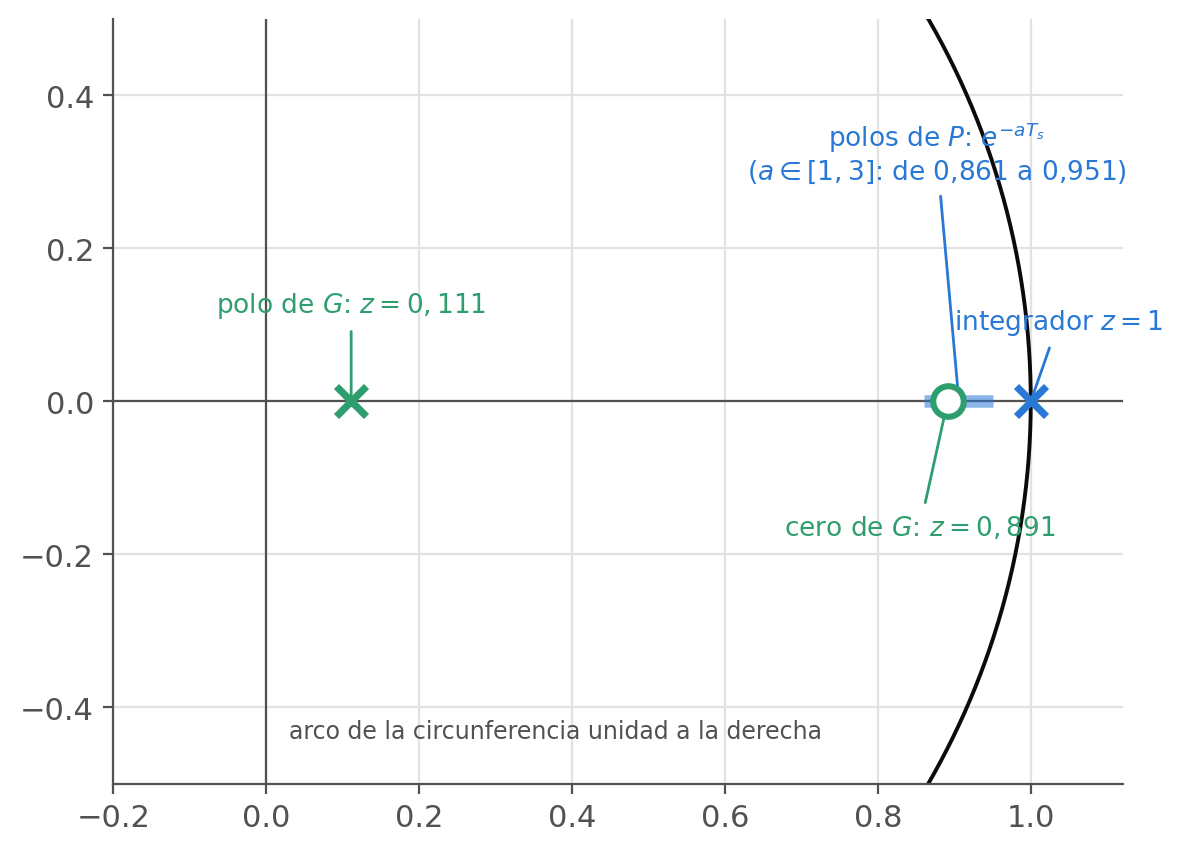
\includegraphics[width=\textwidth]{fig/polos_z.png}
  \end{column}
  \begin{column}{0.48\textwidth}
    El adelanto resultante es
    \[ G(z)=\frac{40.87-36.43\,z^{-1}}{1-0.111\,z^{-1}} \]
    con un cero en $z=0.891$ y un polo en $z=0.111$.
    \begin{itemize}
      \item El \textbf{cero} cae entre los polos de la planta $e^{-aT_s}\in[0.861,0.951]$, igual que el cero $s=-2.3$ caía entre los polos $a\in[1,3]$.
      \item El \textbf{polo} cerca del origen ($z=0.111$) es un polo \emph{rápido}: la dinámica que añade se apaga en pocos periodos. Un cero cerca de $1$ es \emph{lento}.
    \end{itemize}
    Es el mismo adelanto, visto con otra regla: cero lento y polo rápido dan fase positiva en la zona del cruce.
  \end{column}
  \end{columns}
\end{frame}

\section{Camino w}
\begin{frame}{Camino $w$: la planta en el plano $w$}
  \footnotesize
  \begin{columns}[T]
  \begin{column}{0.5\textwidth}
    Sustituyendo $z=\frac{1+T_sw/2}{1-T_sw/2}$ en $P(z)$ queda una función racional de $w$:
    \[ P(w)\approx\frac{K\,(1-w/40)}{w\,(w+a)} \]
    \begin{itemize}
      \item Mismos polos que $P(s)$ ($0$ y $\approx-a$).
      \item Un \textbf{cero en el semiplano derecho} exactamente en $w=2/T_s=40$: es el ZOH.
      \item Otro cero muy lejos ($\approx-4800$), irrelevante.
    \end{itemize}
    Fase extra frente a $P(s)$: $-\arctan(\nu/40)$: $-13.9^\circ$ en $\nu=10$, $-44.5^\circ$ en $\nu=40$.
  \end{column}
  \begin{column}{0.48\textwidth}
    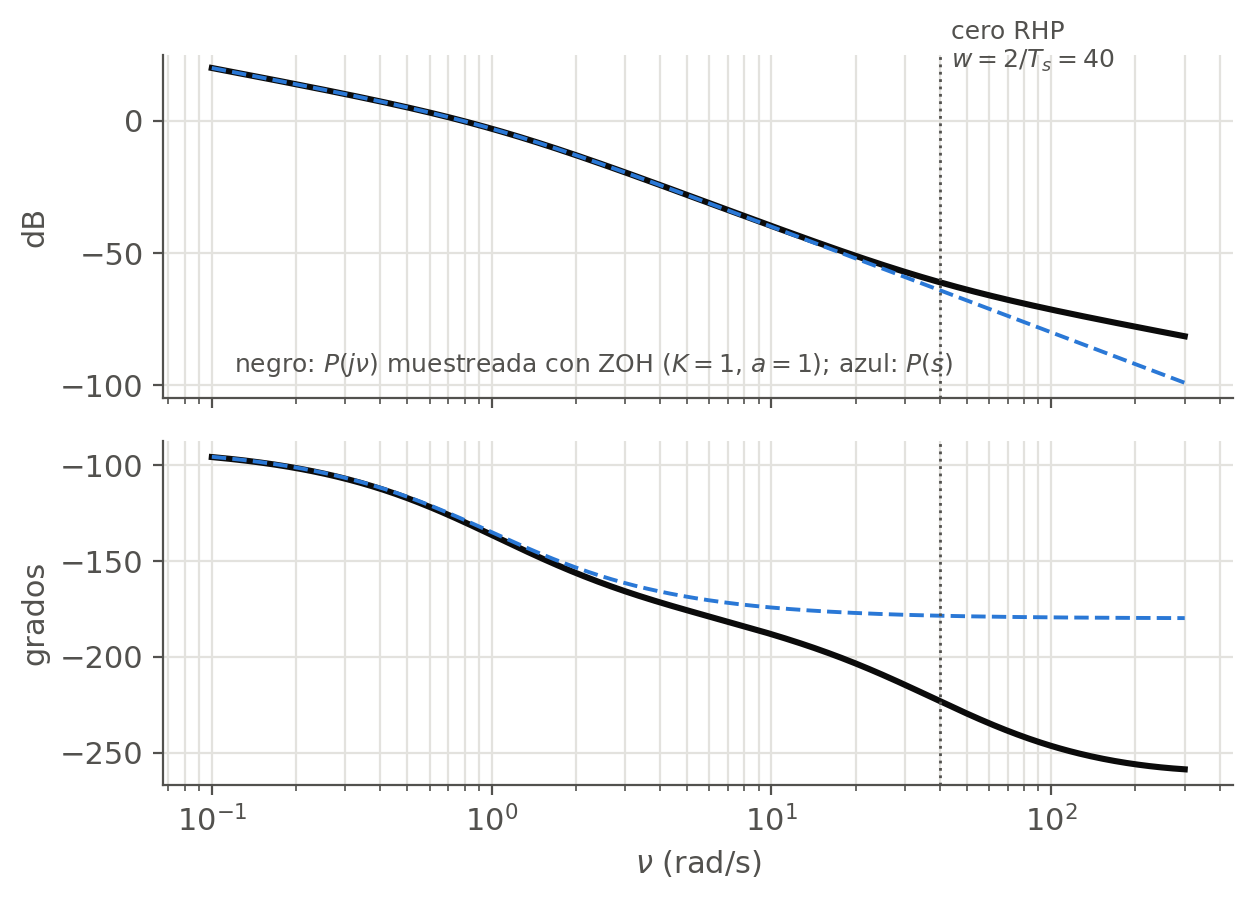
\includegraphics[width=\textwidth]{fig/planta_w.png}
  \end{column}
  \end{columns}
\end{frame}

\begin{frame}{Camino $w$: el loop shaping vuelve a ser de Bode}
  \footnotesize
  \begin{columns}[T]
  \begin{column}{0.58\textwidth}
    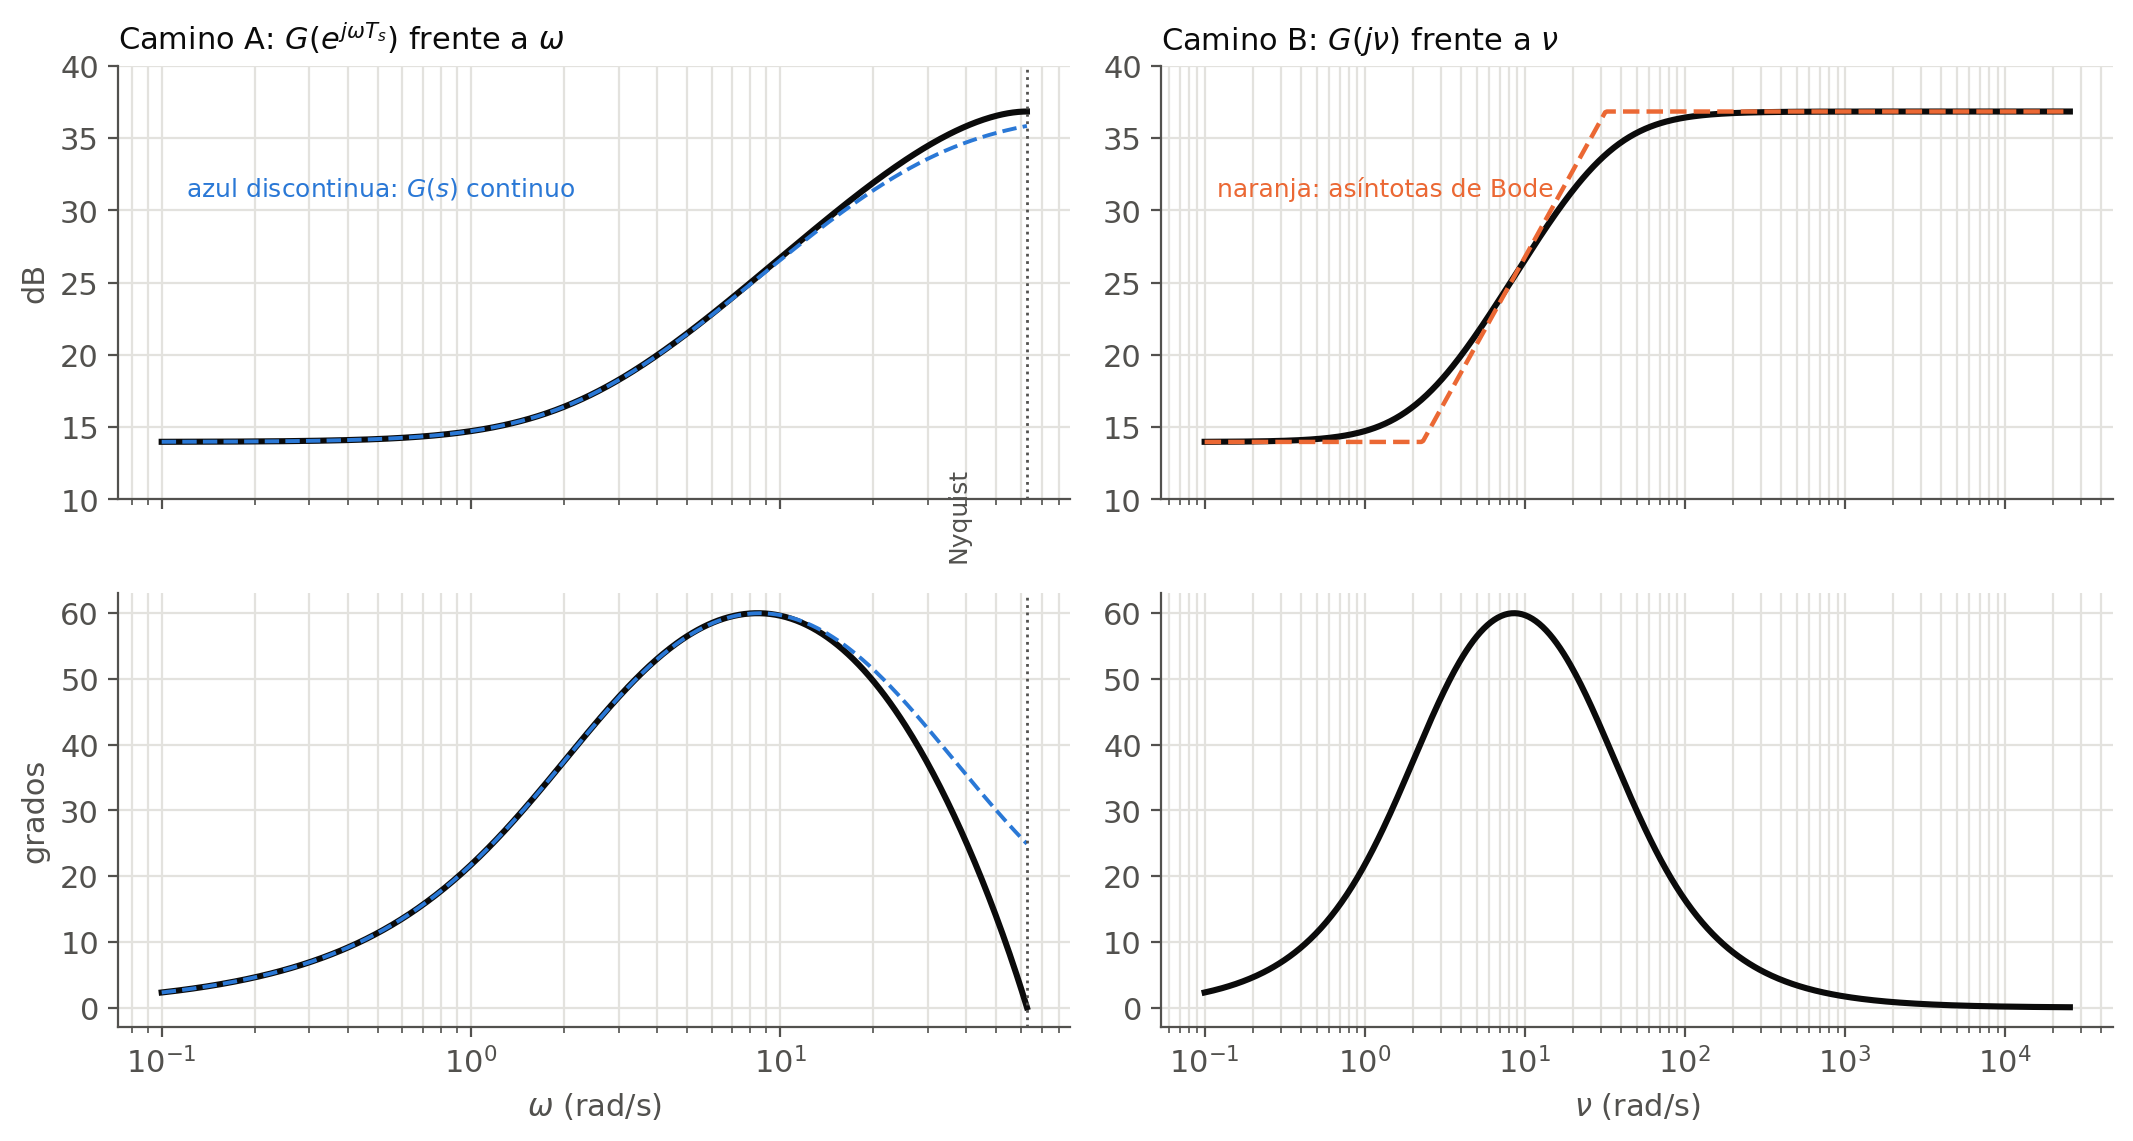
\includegraphics[width=\textwidth]{fig/bode_zw.png}
  \end{column}
  \begin{column}{0.4\textwidth}
    Derecha: el \textbf{mismo} $G$ frente a $\nu$. Ahora son rectas:
    \[ G(w)=5\,\frac{1+w/2.3}{1+w/32} \]
    \begin{itemize}
      \item Ganancia $5$ ($14$ dB) hasta el cero en $\nu=2.3$.
      \item Sube $+20$ dB/dec hasta el polo en $\nu=32$.
      \item Plano de nuevo en $69.6$ ($36.8$ dB).
      \item Fase máxima $+60^\circ$ cerca de $\nu\approx8.5$.
    \end{itemize}
    Las reglas del paso 9 (ganancia, cero, polo) se aplican tal cual.
  \end{column}
  \end{columns}
\end{frame}

\begin{frame}{Camino $w$: de $G(w)$ a $G(z)$}
  \small
  \begin{block}{Sustitución exacta}
    $G(z)=G(w)\big|_{w=\frac{2}{T_s}\frac{z-1}{z+1}}$. Es la transformación de Tustin, pero aplicada a un $G$ diseñado \textbf{en $w$}, así que no se pierde nada.
  \end{block}
  \[ G(w)=5\,\frac{1+w/2.3}{1+w/32}\ \Rightarrow\ G(z)=\frac{40.87-36.43\,z^{-1}}{1-0.111\,z^{-1}} \]
  y la ecuación en diferencias es
  \[ u_k=0.111\,u_{k-1}+40.87\,e_k-36.43\,e_{k-1} \]
  \begin{alertblock}{Ojo con la diferencia respecto a la emulación del paso 10}
    Allí se diseñaba $G(s)$ contra $P(s)$ \textbf{sin ZOH} y luego se discretizaba. Aquí se diseña $G(w)$ contra $P(w)$, que \textbf{ya incluye} el ZOH y el eje $\nu$. Es el mismo Tustin con otro problema de diseño.
  \end{alertblock}
\end{frame}

\begin{frame}{Pre-warping: las especificaciones están en $\omega$, el diseño en $\nu$}
  \footnotesize
  \begin{columns}[T]
  \begin{column}{0.5\textwidth}
    Las especificaciones ($T_L$, $T_U$, $W_d$) se dan en rad/s \textbf{reales}. Si el diseño se hace en $\nu$:
    \begin{enumerate}
      \item Se elige una frecuencia real $\omega_k$.
      \item Se calcula $\nu_k=\frac{2}{T_s}\tan\frac{\omega_kT_s}{2}$.
      \item Se evalúa $P_i(j\nu_k)$ y se calcula el bound ahí, pero con las \textbf{especificaciones de $\omega_k$}.
      \item En el Nichols se compara con $L_0(j\nu_k)$.
    \end{enumerate}
  \end{column}
  \begin{column}{0.48\textwidth}
    \begin{alertblock}{Error típico}
      Usar $\omega_k$ como $\nu_k$. Con $T_s=0.05$ s, el bound de $\omega=40$ se calcularía en $\nu=40$, que en realidad corresponde a $\omega=31.4$ rad/s (un $21\%$ más bajo). A baja frecuencia casi no se nota; en la zona de $\omega\gtrsim20$ sí.
    \end{alertblock}
    \begin{block}{Regla}
      Frecuencias de diseño siempre en $\omega$; se convierte a $\nu$ solo para evaluar las funciones racionales.
    \end{block}
  \end{column}
  \end{columns}
\end{frame}

\section{Resultado}
\begin{frame}{El mismo punto en el Nichols, con las dos etiquetas}
  \footnotesize
  \begin{columns}[T]
  \begin{column}{0.64\textwidth}
    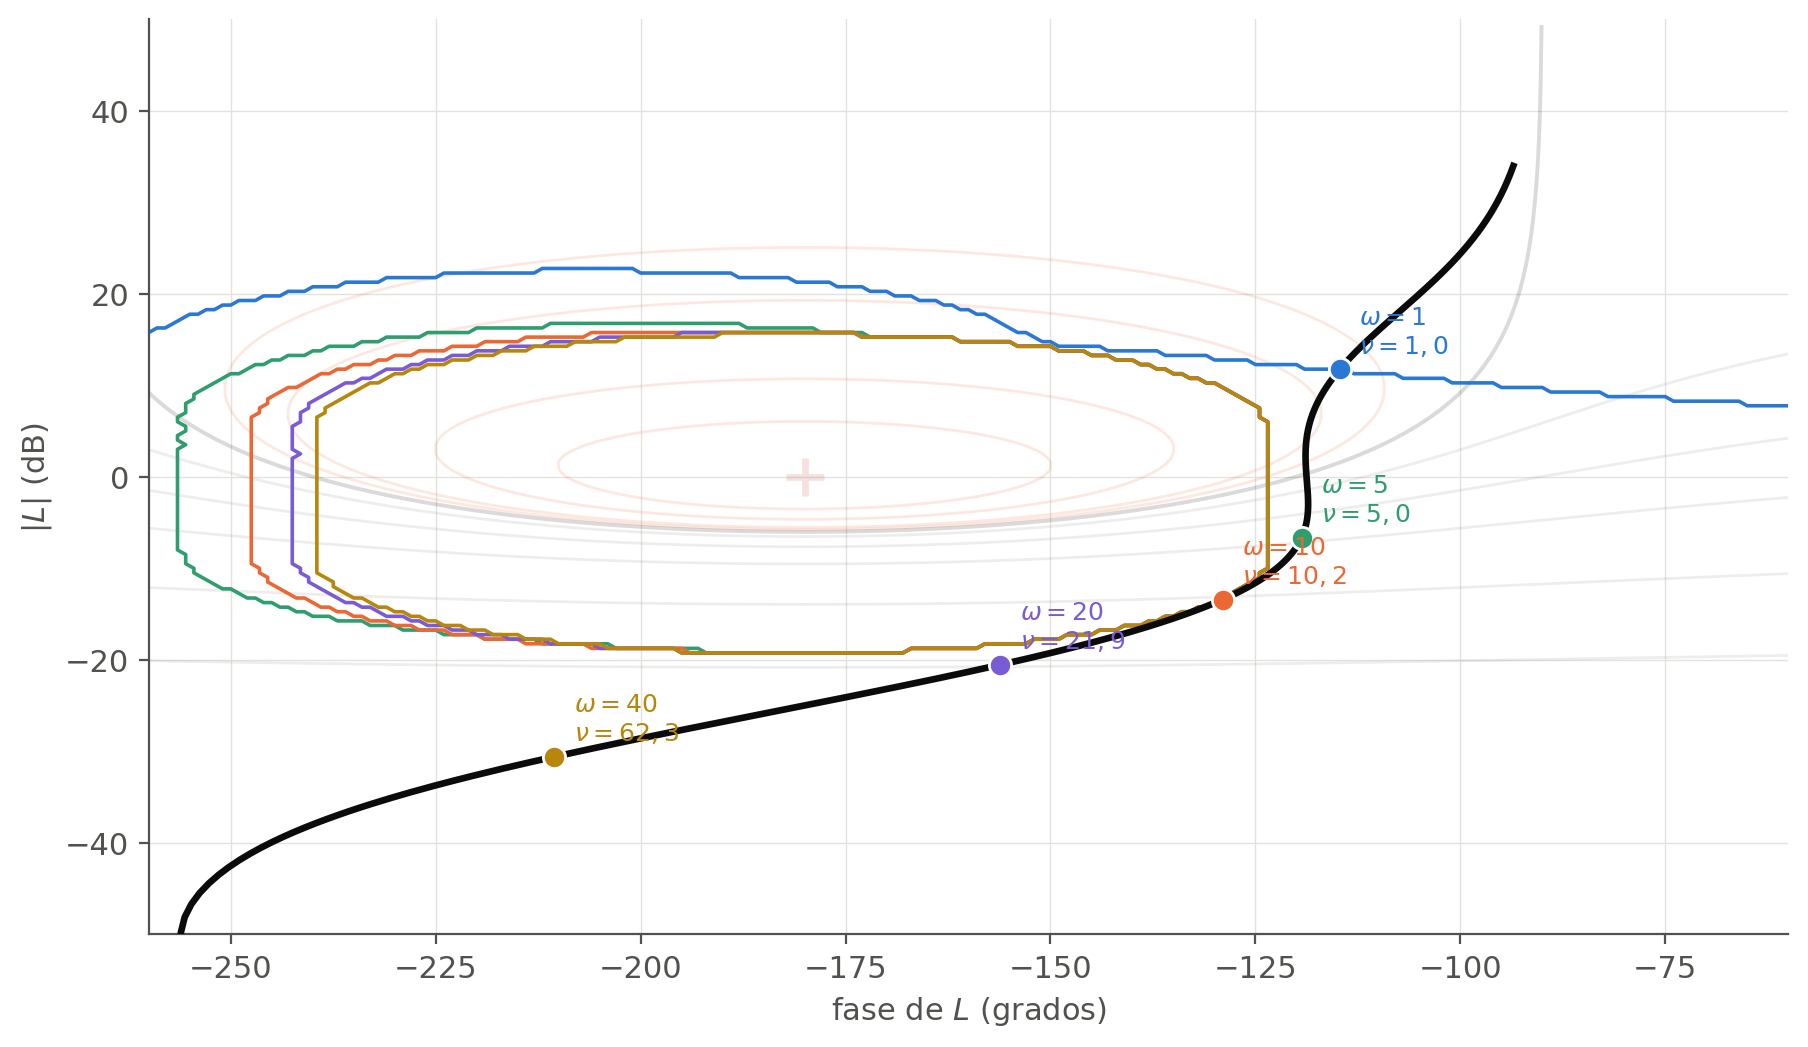
\includegraphics[width=\textwidth]{fig/nichols_dual.png}
  \end{column}
  \begin{column}{0.34\textwidth}
    $L_0=G\,P_0$ con $G(w)=5\frac{1+w/2.3}{1+w/32}$. Cada punto lleva su $\omega$ y su $\nu$.
    \begin{itemize}
      \item Los contornos son los bounds en $\omega=1,5,10,20,40$ (digitales, con $P_i(z)$).
      \item El nominal queda en el lado permitido en las cinco frecuencias.
      \item En $\omega=40$: $\nu=62.3$.
    \end{itemize}
    La carta es la \textbf{misma} para los dos caminos.
  \end{column}
  \end{columns}
\end{frame}

\begin{frame}{Verificación en frecuencia (toda la familia, hasta Nyquist)}
  \small
  Rejilla densa de unas 300 frecuencias hasta $0.995\,\omega_N$, más $\omega=0.5$, $1$ y $2$; $221$ plantas:
  \begin{center}
  \begin{tabular}{l|c|c|c}
    Especificación & Requisito & Obtenido & ¿Cumple?\\\hline
    Estabilidad $\max|T_i|$ & $\le1.58$ dB & $1.56$ dB & sí (justo)\\
    Perturbación $|S|$, $\omega\le0.5$ & $\le0.3$ & $0.283$ & sí\\
    Perturbación $|S|$, $0.5<\omega\le1$ & $\le0.5$ & $0.495$ & sí\\
    Seguimiento (banda con $F$), $\omega\le40$ & dentro de $T_L$--$T_U$ & margen $0.02$ dB & sí (justo)\\
    Margen de fase mínimo & -- & $49.5^\circ$ & --\\
    Margen de ganancia mínimo & -- & $11.1$ dB & --
  \end{tabular}
  \end{center}
  \begin{block}{Lectura}
    Cumple las especificaciones con poco margen (el diseño se ha ajustado al límite del $T_s$). Para $\omega>40$ el seguimiento ya no se exige: cerca de Nyquist $|T|$ cae más rápido que $T_L$ por el cero del ZOH.
  \end{block}
\end{frame}

\begin{frame}{Verificación en el tiempo}
  \footnotesize
  \begin{columns}[T]
  \begin{column}{0.6\textwidth}
    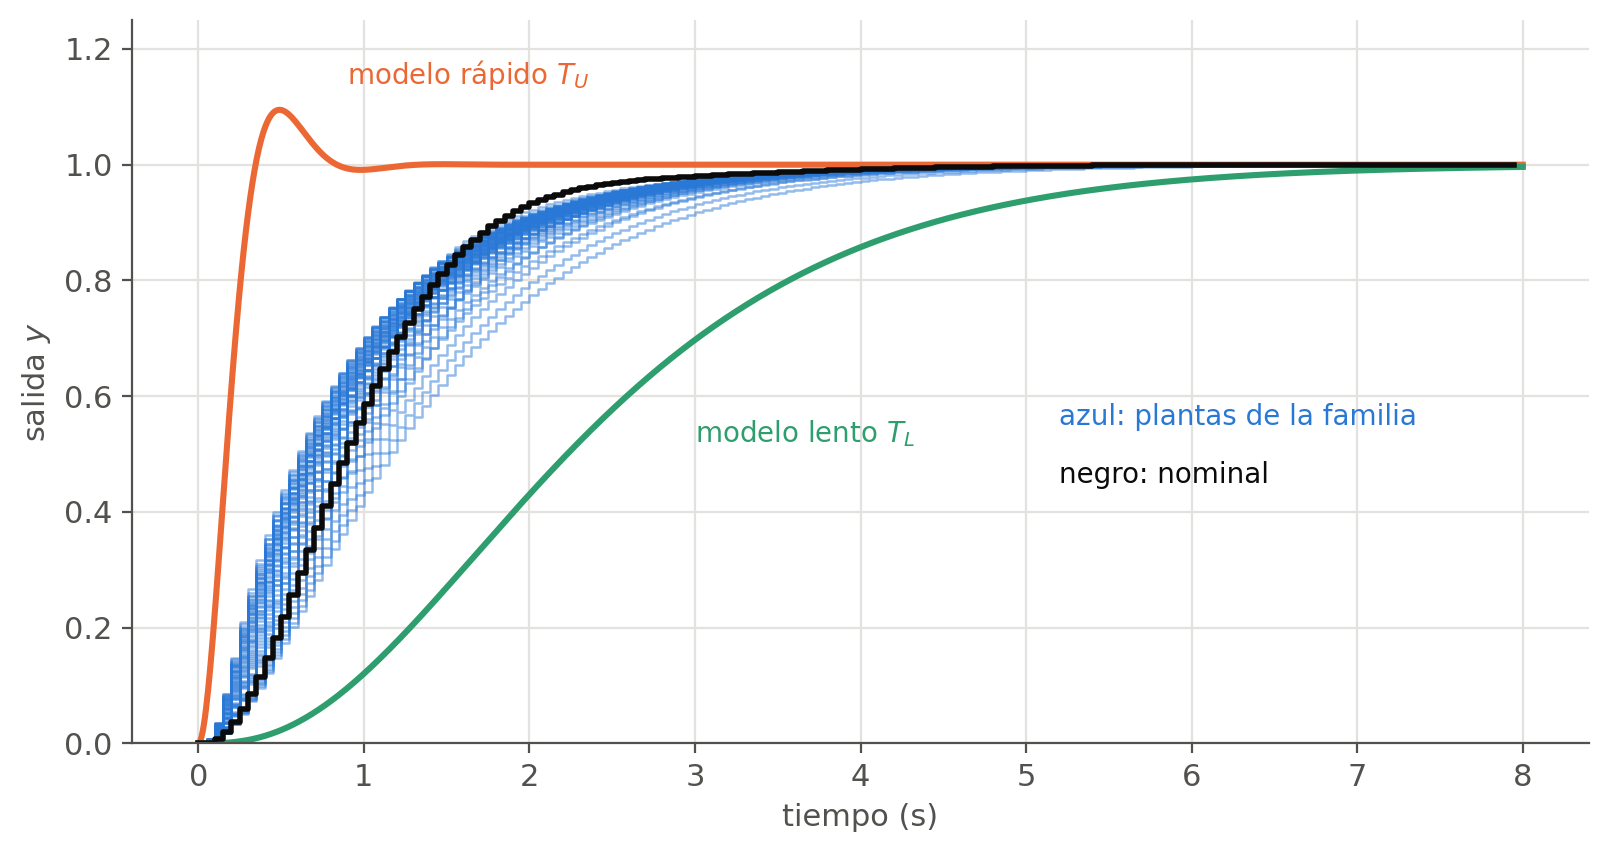
\includegraphics[width=\textwidth]{fig/escalon_dig2.png}
  \end{column}
  \begin{column}{0.38\textwidth}
    Respuesta a un escalón en $r$ con el prefiltro digital $F(z)$ ($F(s)=\frac{1.2}{s+1.2}$ con Tustin) y $T_s=0.05$ s, para $K\in\{1,\dots,5\}$, $a\in\{1,\dots,3\}$.
    \begin{itemize}
      \item Todas quedan entre el modelo rápido $T_U$ y el lento $T_L$.
      \item Ninguna pasa de $1.0$ (sin sobreoscilación).
    \end{itemize}
    \alert{Solo se ven los instantes de muestreo}; entre muestras la salida de la planta continua puede tener un rizado que esta figura no muestra.
  \end{column}
  \end{columns}
\end{frame}

\begin{frame}{Comparativa de los dos caminos}
  \footnotesize
  \begin{center}
  \begin{tabular}{p{2.6cm}|p{4.2cm}|p{4.8cm}}
     & \textbf{Camino $z$} & \textbf{Camino $w$}\\\hline
    Eje de frecuencia & $\omega\in(0,\omega_N]$, real & $\nu\in(0,\infty)$, deformado\\[2pt]
    $G$ & polos/ceros en el círculo unidad ($0.891$ y $0.111$) & polos/ceros reales ($2.3$ y $32$)\\[2pt]
    Reglas de Bode & no valen & sí valen\\[2pt]
    ZOH & dentro de $P(z)$ & cero en $w=2/T_s$\\[2pt]
    Especificaciones & se evalúan en $\omega$ & hay que convertir $\omega\to\nu$\\[2pt]
    Nichols & mismos puntos & mismos puntos\\[2pt]
    Salida & $G(z)$ directamente & $G(w)\to G(z)$ por sustitución
  \end{tabular}
  \end{center}
\end{frame}

\begin{frame}{Cuál usar}
  \small
  \begin{block}{Receta recomendada}
    \textbf{Diseñar en $w$, verificar en $z$.} La intuición de Bode sirve para dar forma al lazo; la verificación final se hace siempre con $L(e^{j\omega T_s})$ real hasta Nyquist y en el tiempo.
  \end{block}
  \begin{itemize}
    \item Si el diseño lo hace una optimización (como en este ejemplo para ajustar $k$, $z_0$, $p_0$), da igual el camino: se optimiza $G(z)$ directamente.
    \item Si se diseña a mano, el plano $w$ es mucho más cómodo.
    \item Con $T_s$ pequeño ($\omega_s\gtrsim30\,\omega_c$), $\nu\approx\omega$ en toda la zona útil y los dos caminos casi coinciden con el continuo.
  \end{itemize}
  \begin{alertblock}{Siempre}
    Comprobar también el retardo de cómputo y lo que ocurre entre muestras.
  \end{alertblock}
\end{frame}

\begin{frame}{Ejercicio}
  \small
  Un controlador $G(s)=\dfrac{50(s+2)}{s+20}$ se va a implementar con $T_s=0.1$ s. Se quiere evaluarlo en $\omega=15$ rad/s.
  \begin{enumerate}
    \item ¿Cuánto vale $\nu$ para $\omega=15$? ¿Y $\omega_N$?
    \item Calcula módulo (dB) y fase de $G(w)=\dfrac{50(w+2)}{w+20}$ en $w=j\nu$.
    \item El Tustin de este $G$ es $G(z)=27.5-22.5\,z^{-1}$. Evalúalo en $z=e^{j\omega T_s}$ y comprueba que coincide con el apartado 2.
    \item ¿En cuánto se equivoca quien evalúa $G(s)$ en $s=j15$ en vez de $G(w)$ en $w=j\nu$?
  \end{enumerate}
  \textcolor{gray}{Solución en el apéndice.}
\end{frame}

\begin{frame}{Para programarlo: el notebook de este paso}
  \small
  Todo lo de este paso se puede \textbf{ejecutar} en el notebook \texttt{notebooks/paso11\_dos\_caminos.ipynb}.
  \begin{itemize}
    \item Python: $\nu=\frac{2}{T_s}\tan\frac{\omega T_s}{2}$, la sustitución $z\to w$ de polinomios y la equivalencia numérica de los dos caminos.
    \item Cada cálculo de las diapositivas se \textbf{comprueba} en código, con las mismas cifras.
    \item Incluye celdas \emph{Tu turno} con el ejercicio del paso y la solución plegada.
  \end{itemize}
  \footnotesize Requisitos: \texttt{numpy}, \texttt{scipy}, \texttt{matplotlib}; se abre con \texttt{jupyter lab notebooks/}. Ver \texttt{GUIA.md}.
\end{frame}

\begin{frame}{Resumen}
  \small
  \begin{itemize}
    \item El Bode y el Nichols digitales \textbf{existen}: son $L(e^{j\omega T_s})$ para $\omega\le\omega_N$.
    \item \textbf{Camino $z$}: Nichols directo, sin conversión de frecuencias, pero sin reglas asintóticas.
    \item \textbf{Camino $w$}: $\nu=\frac{2}{T_s}\tan\frac{\omega T_s}{2}$; todo racional, Bode otra vez; el ZOH es un cero en $w=2/T_s$.
    \item Los dos dan los \textbf{mismos puntos} en el Nichols; cambia la etiqueta ($\omega$ o $\nu$).
    \item Especificaciones en $\omega$ real (pre-warping al pasar a $\nu$).
    \item Ejemplo: $G(w)=5\frac{1+w/2.3}{1+w/32}$, $F=\frac{1.2}{s+1.2}$, $T_s=0.05$ s cumple con poco margen.
  \end{itemize}
\end{frame}

\appendix
\begin{frame}\centering\Large Apéndice\end{frame}

\begin{frame}{Solución del ejercicio}
  \footnotesize
  \textbf{1.} $\nu=\dfrac{2}{0.1}\tan\dfrac{15\cdot0.1}{2}=20\tan0.75=18.63$ rad/s. $\omega_N=\pi/0.1=31.4$ rad/s.\\[3pt]
  \textbf{2.} $G(j18.63)=\dfrac{50(2+j18.63)}{20+j18.63}=25.9+j22.4$: módulo $34.28$ ($30.7$ dB), fase $40.9^\circ$.\\[3pt]
  \textbf{3.} $G(e^{j1.5})=27.5-22.5\,e^{-j1.5}=25.9+j22.4$: es el \textbf{mismo} número complejo.\\[3pt]
  \textbf{4.} $G(j15)=21.2+j21.6$: módulo $30.27$ ($29.6$ dB), fase $45.5^\circ$. Frente al valor correcto, el error es de $-1.1$ dB y $+4.6^\circ$.
  \begin{block}{Lectura}
    Evaluar el Tustin en $\omega$ en lugar de $\nu$ da un error que crece al acercarse a Nyquist. A $\omega=15$ ($\omega T_s=1.5$) ya son casi $5^\circ$.
  \end{block}
\end{frame}

\begin{frame}{Para curiosos: por qué $\nu=\frac{2}{T_s}\tan\frac{\omega T_s}{2}$}
  \small
  Con $z=e^{j\omega T_s}$:
  \[ \frac{z-1}{z+1}=\frac{e^{j\omega T_s/2}-e^{-j\omega T_s/2}}{e^{j\omega T_s/2}+e^{-j\omega T_s/2}}=j\tan\frac{\omega T_s}{2} \]
  \[ \Rightarrow\quad w=\frac{2}{T_s}\,j\tan\frac{\omega T_s}{2}=j\nu \]
  \begin{block}{El cero del ZOH, exacto en un integrador}
    $P(s)=\frac{1}{s}$ con ZOH da $P(z)=\frac{T_s}{z-1}$. Con $z-1=\frac{T_sw}{1-T_sw/2}$ queda
    \[ P(w)=\frac{1-T_sw/2}{w} \]
    un cero exacto en $w=2/T_s$ cuya fase es $-\arctan(\nu T_s/2)=-\omega T_s/2$, justo el retardo de $T_s/2$ del paso 10.
  \end{block}
\end{frame}
\end{document}
